For the initial Denial of Service simulation, the network topology is as shown
in Figure \ref{fig:dosNetwork}. This network consists of an attacking traffic
source (shown on the left), a legitimate user traffic source (shown on the
right), and a server (shown on the bottom).

\begin{figure}[H]
	\centering
	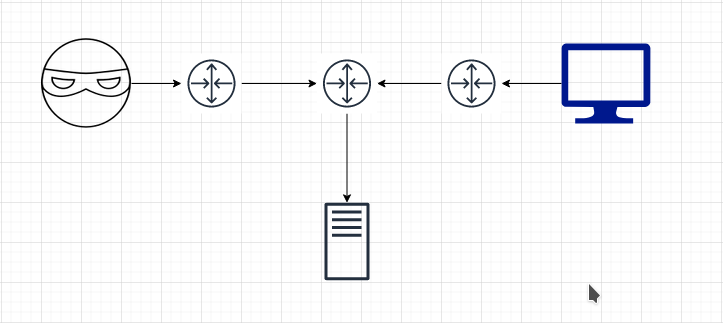
\includegraphics[width=0.8\textwidth]{images/dosNetwork}
	\caption{Denial of Service Network Topology}
	\label{fig:dosNetwork}
\end{figure}

As an initial attack, the "hping" tool is used. Hping is a tool for creating and
transmitting TCP, UDP or ICMP packets. This tool has multiple functions, such as
port scanning, and firewall mapping, but can also be utilised as a Denial of
Service tool. By utilising the tools "rand-source" and "flood" flags, the tool
can execute a SYN flood, sending TCP SYN packets to the target address via
spoofed IP addresses.
